\documentclass{article}
\usepackage{amsmath}
\usepackage{amssymb}
\usepackage{xargs}
\usepackage[dvipsnames]{xcolor}
\usepackage[margin=1.2in]{geometry}
\usepackage{graphicx}
\usepackage{tikz}
\usepackage{pgfplots, pgfplotstable}
\usetikzlibrary{arrows}
\usetikzlibrary{datavisualization.formats.functions}
\usepgfplotslibrary{fillbetween}
\usetikzlibrary{patterns}

\begin{document}

\title{Differential Equations HW \#1}
\author{Ozaner Hansha}
\date{September 19, 2019}
\maketitle

\newcommandx{\der}[2][1=y, 2=t]{\frac{d#1}{d#2}}

\section*{Problem 1}
\noindent\textbf{Part a:} Solve the following differential equation:

\begin{equation*}
    y'=t^4y
\end{equation*}

\noindent\textbf{Solution:} The solution set is given by the following chain of equalities:

\begin{align*}
    \der&=t^4y\\
    \int \frac{1}{y}\mathop{dy}&=\int t^4\mathop{dt}\tag{separable equation}\\
    \ln{|y|}&=\frac{t^5}{5}+C_1\tag{integration}\\
    |y|&=e^{\frac{t^5}{5}}e^{C_1}\tag{exponentiation}\\
    y&=C_2e^{\frac{t^5}{5}}\tag{$\pm e^{C_1}=C_2\not=0$}
\end{align*}

Note that by letting $C_2=0$, we arrive at what happens to be the sole equilibrium solution: $y=0$. Thus we can replace $C_2$ with a new constant $C_3$ that can take on any real value. This gives us the following family of solutions indexed by $C\in\mathbb R$:

\begin{equation*}
    y(t)=Ce^{\frac{t^5}{5}}
\end{equation*}
\smallskip

\noindent\textbf{Part b:} Solve the following differential equation:

\begin{equation*}
    y'=2y+1
\end{equation*}

\noindent\textbf{Solution:} The solution set is given by the following chain of equalities:

\begin{align*}
    \der&=2y+1\\
    \int \frac{1}{2y+1}\mathop{dy}&=\int\mathop{dt}\tag{separable equation}
\end{align*}
\pagebreak

At this point we perform $u$-substitution on the LHS:
\begin{gather*}
    u=2y+1\\
    \der[u][y]=2\implies dy=\frac{du}{2}
\end{gather*}

Plugging this into our integral we find:

\begin{align*}
    \int \frac{1}{2u}\mathop{du}&=\int\mathop{dt}\tag{$u$-substitution}\\
    \frac{1}{2}\ln{|u|}&=t+C_1\tag{integration}\\
    \frac{1}{2}\ln{|2y+1|}&=t+C_1\tag{$u$-substitution}\\
    \ln{|2y+1|}&=2t+C_2\tag{algebra}\\
    |2y+1|&=e^{2t}e^{C_2}\tag{exponentiation}\\
    2y+1&=C_3e^{2t}\tag{$\pm e^{C_2}=C_3\not=0$}\\
    y&=C_4e^{2t}-\frac{1}{2}\tag{algebra}
\end{align*}

Note that by letting $C_4=0$, we arrive at what happens to be the sole equilibrium solution: $y=-\frac{1}{2}$. Thus we can replace $C_4$ with a new constant $C$ that can take on any real value. This gives us the following family of solutions indexed by $C\in\mathbb R$:

\begin{equation*}
    y(t)=Ce^{2t}-\frac{1}{2}
\end{equation*}
\smallskip

\noindent\textbf{Part c:} Solve the following differential equation:

\begin{equation*}
    y'=\frac{t}{t^2y+y}
\end{equation*}
\smallskip

\noindent\textbf{Solution:} The solution set is given by the following chain of equalities:

\begin{align*}
    \der&=\frac{t}{t^2y+y}\\
    &=\frac{t}{y(t^2+1)}\tag{algebra}\\
    \int y\mathop{dy}&=\int \frac{t}{t^2+1}\mathop{dt}\tag{separable equation}\\
\end{align*}

At this point we perform $u$-substitution on the RHS:
\begin{gather*}
    u=t^2+1\\
    \der[u]=2t\implies dt=\frac{du}{2t}
\end{gather*}

Plugging this into our integral we find:
\begin{align*}
    \int y\mathop{dy}&=\int \frac{t}{2tu}\mathop{du}\tag{$u$-substitution}\\
    \int y\mathop{dy}&=\frac{1}{2}\int\frac{1}{u}\mathop{du}\tag{algebra}\\
    \frac{y^2}{2}&=\frac{1}{2}\ln{|u|}+C_1\tag{integration}\\
    \frac{y^2}{2}&=\frac{1}{2}\ln{|t^2+1|}+C_1\tag{$u$-substitution}\\
    y&=\pm\sqrt{\ln{|t^2+1|}+C_2}\tag{algebra}
\end{align*}

And so we have the following family of solutions with each one given by a constant $C_2\in\mathbb R$ and a choice of $+$ or $-$:

\begin{equation*}
    y(t)=\pm\sqrt{\ln{|t^2+1|}+C_2}
\end{equation*}

\section*{Problem 2}
\noindent\textbf{Part a:} Solve the following IVP:

\begin{equation*}
    y'=t^2y^3,\,\,\,\, y(0)=-1
\end{equation*}
\smallskip

\noindent\textbf{Solution:} First we must find the solution set of the differential equation:

\begin{align*}
    \der&=t^2y^3\\
    \int \frac{1}{y^3}\mathop{dy}&=\int t^2\mathop{dt}\tag{separable equation}\\
    -\frac{1}{2y^2}&=\frac{t^3}{3}+C_1\tag{integration}\\
    \frac{1}{y^2}&=-\frac{2t^3}{3}+C_2\tag{algebra}\\
    y&=\pm\sqrt{\frac{1}{-\frac{2t^3}{3}+C_2}}\tag{algebra}
\end{align*}

Now by plugging in our initial condition we can solve for the constant $C_2$ that corresponds to our partiular solution:

\begin{align*}
    -1&=\pm\sqrt{\frac{1}{-\frac{2\cdot0^3}{3}+C_2}}\tag{$(t,y)=(0,-1)$}\\
    &=\pm\sqrt{\frac{1}{C_2}}\\
    &=-\sqrt{\frac{1}{C_2}}\tag{$+$ case impossible}\\
    \implies C_2&=1
\end{align*}

And so our constant $C_2=1$ and our choice of sign is $-$, giving us the following solution:

\begin{equation*}
    y(t)=-\sqrt{\frac{1}{-\frac{2t^3}{3}+1}}
\end{equation*}
\bigskip

\noindent\textbf{Part b:} Solve the following IVP:

\begin{equation*}
    y'=\frac{1-y^2}{y},\,\,\,\, y(0)=-2
\end{equation*}
\smallskip

\noindent\textbf{Solution:} First we must find the solution set of the differential equation:

\begin{align*}
    \der&=\frac{1-y^2}{y}\\
    \int\frac{y}{1-y^2}\mathop{dy}&=\int\mathop{dt}\tag{separable equation}\\
\end{align*}

At this point we perform $u$-substitution on the LHS:
\begin{gather*}
    u=1-y^2\\
    \der[u][y]=-2y\implies dy=\frac{du}{-2y}
\end{gather*}

Plugging this into our integral we find:

\begin{align*}
    \int\frac{y}{-2yu}\mathop{du}&=\int\mathop{dt}\tag{$u$-substitution}\\
    -\frac{1}{2}\int\frac{1}{u}\mathop{du}&=\int\mathop{dt}\tag{algebra}\\
    -\frac{1}{2}\ln|u|&=t+C_1\tag{integration}\\
    -\frac{1}{2}\ln|1-y^2|&=t+C_1\tag{$u$-substitution}\\
    \ln|1-y^2|&=-2t+C_2\tag{algebra}\\
    |1-y^2|&=e^{-2t}e^{C_2}\tag{exponentiation}\\
    1-y^2&=C_3e^{-2t}\tag{$\pm e^{C_2}=C_3\not=0$}\\
    y&=\pm\sqrt{C_4e^{-2t}+1}\tag{algebra}
\end{align*}

Now by plugging in our initial condition we can solve for the constant $C_4$ that corresponds to our partiular solution:
\begin{align*}
    -2&=\pm\sqrt{C_4e^{-2\cdot0}+1}\tag{$(t,y)=(0,-2)$}\\
    &=\pm\sqrt{C_4+1}\\
    &=-\sqrt{C_4+1}\tag{$+$ case impossible}\\
    \implies C_4&=3
\end{align*}

And so our constant $C_4=3$ and our choice of sign is $-$, giving us the following particular solution:

\begin{equation*}
    y(t)=-\sqrt{3e^{-2t}+1}
\end{equation*}

\section*{Problem 3}
A cup of hot chocolate is initially $170\,{^\circ\text{F}}$ and is left in a room with an ambient temperature of $70\,{^\circ\text{F}}$. Suppose that at time $t=0$ it is cooling at a rate of $20\,{^\circ\text{F}}$ per minute.
\bigskip

\noindent\textbf{Part a:} Assume that the rate of cooling is proportional to the difference between the current temperature and the ambient temperature (Newton's cooling law). Write an initial value problem that models the temperature of the hot chocolate.
\bigskip

\noindent\textbf{Solution:} Letting $y$ be the temperature of the hot chocolate and $T$ the ambient temperature, Newton's law of cooling is given by:

\begin{equation*}
    \der=-k(y-T)
\end{equation*}

For some constant $k$. Plugging in $y=170$, $T=70$, and setting the derivative equal to $-20$ (as per the initial condition) we get:

\begin{equation*}
    \der=k(170-70)=-20\implies k=-\frac{1}{5}\\    
\end{equation*}
\smallskip

Now plugging in these values for $T$ and $k$ we have:

\begin{align*}
    \der&=-\frac{(y-70)}{5}\\
    \int-\frac{5}{y-70}\mathop{dy}&=\int\mathop{dt}\tag{separable equation}\\
    -5\ln|y-70|&=t+C_1\tag{integration}\\
    \ln|y-70|&=-\frac{t}{5}+C_2\tag{algebra}\\
    |y-70|&=e^{-\frac{t}{5}}e^{C_2}\tag{exponentiation}\\
    y-70&=C_3e^{-\frac{t}{5}}\tag{$\pm e^{C_2}=C_3\not=0$}\\
    y&=C_3e^{-\frac{t}{5}}+70\tag{algebra}
\end{align*}

Now by plugging in our initial condition we can solve for the constant $C_3$ that corresponds to our partiular solution:
\begin{align*}
    170&=C_3e^{-\frac{0}{5}}+70\tag{$(t,y)=(0,170)$}\\
    &=C_3+70\\
    \implies C_3&=100
\end{align*}

And so $C_3=100$, giving us the following particular solution:

\begin{equation*}
    y(t)=100e^{-\frac{t}{5}}+70
\end{equation*}

\bigskip

\noindent\textbf{Part b:}  How long does it take the hot chocolate to cool to a temperature of $110\,{^\circ\text{F}}$?
\bigskip

\noindent\textbf{Solution:} Plugging in $110$ into the model of the hot chocolate's temperature we found in part a we have:
\begin{align*}
    100e^{-\frac{t}{5}}+70&=110\tag{$y(t)=110$}\\
    e^{-\frac{t}{5}}&=\frac{2}{5}\tag{algebra}\\
    -\frac{t}{5}&=\ln\left(\frac{2}{5}\right)\tag{$\ln()$ both sides}\\    
    t&=-5\ln\left(\frac{2}{5}\right)\approx4.581\tag{algebra}
\end{align*}

And so the hot chocolate should cool to $110\,{^\circ\text{F}}$ in about 4.581 seconds.

\section*{Problem 4}
Consider the following differential equation:
\begin{equation*}
    y'=f(t,y)=-y^2+y+2yt^2+2t-t^2-t^4
\end{equation*}
\smallskip

\noindent\textbf{Part a:} Show that $y_1(t)=t^2$ and $y_2(t)=t^2+1$ are solutions to the differential equation:
\bigskip

\noindent\textbf{Solution:} Plugging $y_1$ into the differential equation gives us:

\begin{equation*}
    f(t,y_1)=-(t^2)^2+t^2+2(t^2)t^2+2t-t^2-t^4=2t
\end{equation*}

And indeed, this coincides with the derivative of $y_1$:

\begin{equation*}
    y_1'=\der[]t^2=2t
\end{equation*}

Plugging $y_2$ into the differential equation gives us:

\begin{equation*}
    f(t,y_2)=-(t^2+1)^2+t^2+1+2(t^2+1)t^2+2t-t^2-t^4=2t
\end{equation*}

Like before, this coincides with the derivative of $y_2$:

\begin{equation*}
    y_2'=\der[](t^2+1)=2t
\end{equation*}
\smallskip

\noindent\textbf{Part b:} Show that if $y(t)$ is a solution to the differential equation and $0<y(0)<1$, then $t^2<y(t)<t^2+1$ for all $t$.
\bigskip

\noindent\textbf{Solution:} First we compute the partial derivative of $f(t,y)$ with respect to $y$:

\begin{equation*}
    \frac{\partial f}{\partial y}=-2y+1+2t^2
\end{equation*}

Notice that $\frac{\partial f}{\partial y}$ is, for all $t$ and $y$, a continuous function. As a result, the uniqueness theorem applies to solutions of $f(t,y)$. We already know from part a that both $y_1(t)=t^2$ and $y_2(t)=t^2+1$ are solutions to $f$. Graphing them we see:

\pgfplotstableset{
    create on use/x/.style={
        create col/expr={
            \pgfplotstablerow/201*2-1
        }
    },
    create on use/y/.style={
        create col/expr accum={
            \pgfmathaccuma+(2/201)*(abs(\pgfmathaccuma^2)+abs(\thisrow{x}^2)-1)
        }{0.6}
    }
}
\pgfplotstablenew{201}\loadedtable

\begin{center}
    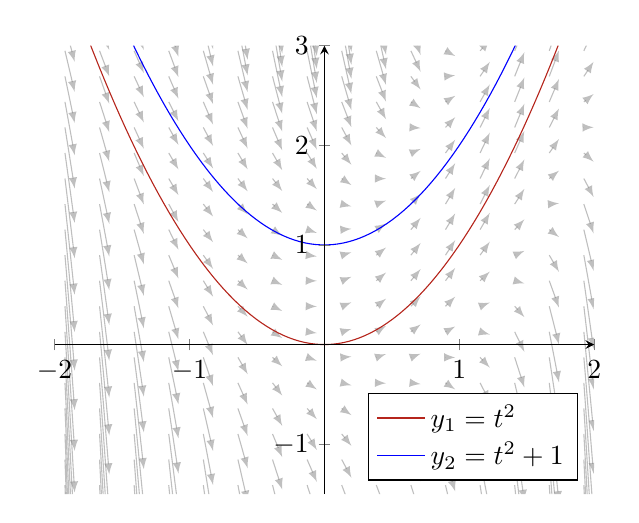
\begin{tikzpicture}
    \begin{axis}[
        view={0}{90},
        xmin=-2,xmax=2,
        axis lines=center,
        ymin=-1.5,ymax=3,
        samples=40,
        legend pos = south east,
        legend style={legend cell align=left,legend plot pos=left}]; 
    \addplot3 [gray,forget plot, opacity=0.5, quiver={u={.9}, v={y-y^2+2*y*x^2+2*x-x^2-x^4}, scale arrows=0.08, every arrow/.append style={-latex}}] (x,y,0);
    \addplot[color=BrickRed,domain=-2:2,samples=100] {x^2};
    \addlegendentry{$y_1=t^2$}
    \addplot[color=blue,domain=-2:2,samples=100] {x^2+1};
    \addlegendentry{$y_2=t^2+1$}
    \end{axis}
    \end{tikzpicture}
\end{center}

Notice that that any solution $y(t)$ with $0<y(0)<1$ is bounded above by $y_2$ and below by $y_1$. This is because $y(t)$ is continuous and cannot intersect any other solution (namely $y_1$ and $y_2$) as that would mean the two solutions solve the same IVP, violating uniqueness. Thus if a solution is between any other two solutions at any time $t_0$, it will be between them for all time $t$. This is all to say that, for any solution $y(t)$ to $f(t,y)$:

\begin{align*}
    y_1(0)<y(0)<y_2(0)&\implies \forall t(y_1(t)<y(t)<y_2(t))\\
    0<y(0)<1&\implies \forall t(t^2<y(t)<t^2+1)
\end{align*}

\section*{Problem 5}
Consider the following differential equation:
\begin{equation*}
    y'=f(t,y)=ty^{\frac{2}{3}}
\end{equation*}

\noindent\textbf{Part a:} Show that $y_1(t)=0$ is a solution to the differential equation:
\bigskip

\noindent\textbf{Solution:} Letting $y=y_1=0$, the differential equation gives us:

\begin{equation*}
    f(t,y_1)=t\cdot0^{\frac{2}{3}}=0
\end{equation*}

And indeed, this coincides with the derivative of $y_1$:

\begin{equation*}
    y_1'=\der[]0=0
\end{equation*}
\smallskip

\noindent\textbf{Part b:} Find another function $y(t)$ which also satisfies the differential equation and $y(0) = 0$. Why does it not contradict the uniqueness theorem?
\bigskip
\pagebreak

\noindent\textbf{Solution:} As this is a separable equation, we have the following chain of equalities:
\begin{align*}
    \der&=ty^{\frac{2}{3}}\\
    \int \frac{1}{y^{\frac{2}{3}}}\mathop{dy}&=\int t\mathop{dt}\tag{separable equation}\\
    3\sqrt[3]{y}&=\frac{t^2}{2}+C_1\tag{integration}\\
    y&=\frac{t^6}{216}+C_2\tag{algebra}\\
\end{align*}

Now by plugging in our initial condition we can solve for the constant $C_2$ that corresponds to our partiular solution:
\begin{align*}
    0&=\frac{0^6}{216}+C_2\tag{$(t,y)=(0,0)$}\\
    \implies C_2&=0
\end{align*}

And so $C_2=0$, giving us the following particular solution:

\begin{equation*}
    y(t)=\frac{t^6}{216}
\end{equation*}

You'll notice that both this solution and the equilibrium solution $y_0(t)=0$ both solve the same IVP and thus are not unique. This is because the precondition for uniqueness is for $\frac{\partial f}{\partial y}$ to be continuous over the desired rectangle of uniqueness, and if we calculate this derivative:

\begin{equation*}
    \frac{\partial}{\partial y}ty^{\frac{2}{3}}=\frac{2t}{3\sqrt[3]{y}}
\end{equation*}

We can see that this partial derivative does not exist for any point $(t,0)$. And so, as mentioned before, the existence of two solutions that solve the same IVP with an initial condition of $y(0)=0$ is consistent.

\section*{Problem 6}
Use Euler’s method with the given step size $\Delta t$ to approximate the solution to the given initial value problem over the time interval specified.
\bigskip

\noindent\textbf{Part a:} Approximate $y(3)$ with $\Delta t=1.0$ for the following differential equation:

\begin{equation*}
    y'=(3-y)(y+1),\,\,\,y(0)=4
\end{equation*}
\smallskip

\noindent\textbf{Solution:} Running the method we have:

\begin{center}
\begin{tabular}{c|c|c}
        Step & $t_i$ & $y_i$\\
        \hline
        0 & 0.0 & 4.00\\
        1 & 1.0 & -1.00\\
        2 & 2.0 & -1.00\\
        3 & 3.0 & -1.00\\
\end{tabular}
\end{center}

Giving us $y(3)\approx-1$.

\bigskip

\noindent\textbf{Part b:} Approximate $w(2)$ with $\Delta t=0.5$ for the following IVP:

\begin{equation*}
    w'=(3-w)(w+1),\,\,\,w(0)=0
\end{equation*}
\smallskip

\noindent\textbf{Solution:} Running the method we have:

\begin{center}
\begin{tabular}{c|c|c}
        Step & $t_i$ & $w_i$\\
        \hline
        0 & 0.0 & 0.000\\
        1 & 0.5 & 1.500\\
        2 & 1.0 & 3.375\\
        3 & 1.5 & 2.555\\
        4 & 2.0 & 3.346\\
\end{tabular}
\end{center}

Giving us $w(2)\approx3.346$.

\end{document}